\documentclass[a4paper]{scrartcl}\usepackage[]{graphicx}\usepackage[]{color}
% maxwidth is the original width if it is less than linewidth
% otherwise use linewidth (to make sure the graphics do not exceed the margin)
\makeatletter
\def\maxwidth{ %
  \ifdim\Gin@nat@width>\linewidth
    \linewidth
  \else
    \Gin@nat@width
  \fi
}
\makeatother

\definecolor{fgcolor}{rgb}{0.345, 0.345, 0.345}
\newcommand{\hlnum}[1]{\textcolor[rgb]{0.686,0.059,0.569}{#1}}%
\newcommand{\hlstr}[1]{\textcolor[rgb]{0.192,0.494,0.8}{#1}}%
\newcommand{\hlcom}[1]{\textcolor[rgb]{0.678,0.584,0.686}{\textit{#1}}}%
\newcommand{\hlopt}[1]{\textcolor[rgb]{0,0,0}{#1}}%
\newcommand{\hlstd}[1]{\textcolor[rgb]{0.345,0.345,0.345}{#1}}%
\newcommand{\hlkwa}[1]{\textcolor[rgb]{0.161,0.373,0.58}{\textbf{#1}}}%
\newcommand{\hlkwb}[1]{\textcolor[rgb]{0.69,0.353,0.396}{#1}}%
\newcommand{\hlkwc}[1]{\textcolor[rgb]{0.333,0.667,0.333}{#1}}%
\newcommand{\hlkwd}[1]{\textcolor[rgb]{0.737,0.353,0.396}{\textbf{#1}}}%
\let\hlipl\hlkwb

\usepackage{framed}
\makeatletter
\newenvironment{kframe}{%
 \def\at@end@of@kframe{}%
 \ifinner\ifhmode%
  \def\at@end@of@kframe{\end{minipage}}%
  \begin{minipage}{\columnwidth}%
 \fi\fi%
 \def\FrameCommand##1{\hskip\@totalleftmargin \hskip-\fboxsep
 \colorbox{shadecolor}{##1}\hskip-\fboxsep
     % There is no \\@totalrightmargin, so:
     \hskip-\linewidth \hskip-\@totalleftmargin \hskip\columnwidth}%
 \MakeFramed {\advance\hsize-\width
   \@totalleftmargin\z@ \linewidth\hsize
   \@setminipage}}%
 {\par\unskip\endMakeFramed%
 \at@end@of@kframe}
\makeatother

\definecolor{shadecolor}{rgb}{.97, .97, .97}
\definecolor{messagecolor}{rgb}{0, 0, 0}
\definecolor{warningcolor}{rgb}{1, 0, 1}
\definecolor{errorcolor}{rgb}{1, 0, 0}
\newenvironment{knitrout}{}{} % an empty environment to be redefined in TeX

\usepackage{alltt}
\usepackage{lscape}
\usepackage[section]{placeins}
\usepackage{rotating}
\usepackage[margin=1.0in]{geometry}
\usepackage[table]{xcolor}
\usepackage[hidelinks]{hyperref}
\renewcommand{\textfraction}{0.05}
\renewcommand{\topfraction}{0.8}
\renewcommand{\bottomfraction}{0.8}
\renewcommand{\floatpagefraction}{0.75}
\IfFileExists{upquote.sty}{\usepackage{upquote}}{}
\begin{document}

\title{A Population Genetic Report}


\subtitle {using PopGenReport Version  3.0.4 }

\author{Adamack \& Gruber}
\maketitle

\begin{itemize}
  \item Adamack, A. T., Gruber, B. (2014), PopGenReport: simplifying basic population genetic analyses in R. \emph{Methods in Ecology and Evolution}, 5: 384-387. \href{http://onlinelibrary.wiley.com/doi/10.1111/2041-210X.12158/full}{doi: 10.1111/2041-210X.12158}.
  \item Gruber, B. and Adamack, A. T. (2015), landgenreport: a new r function to simplify landscape genetic analysis using resistance surface layers. \emph{Molecular Ecology Resources}, 15: 1172-1178. \href{http://onlinelibrary.wiley.com/doi/10.1111/1755-0998.12381/full}{doi: 10.1111/1755-0998.12381}.
\end{itemize}


%<<echo=FALSE, results='asis'>>=
%rref <- citation("PopGenReport")
%print(rref[1], style="latex")
%@
  
%<<echo=FALSE, results='asis'>>=
%print(rref[2], style="latex")
%@

\tableofcontents
\newpage


\section{Counts}
This analysis looks at 32 individuals.

\noindent
\newline The mean number of alleles per locus (across all locations): 6


\noindent
\newline The percentage of missing data was 0\%.

\begin{knitrout}
\definecolor{shadecolor}{rgb}{0.969, 0.969, 0.969}\color{fgcolor}
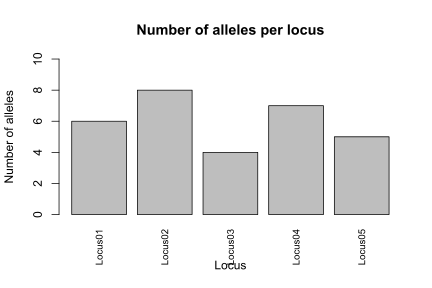
\includegraphics[width=\maxwidth]{PopGenReport-n_alleles_per_locus-1} 

\end{knitrout}
\FloatBarrier



\noindent 
\newline The individuals were sampled from the following locations in the following numbers: 


% latex table generated in R 4.0.4 by xtable 1.8-4 package
% Thu Apr 29 13:49:15 2021
\begin{table}[ht]
\centering
\begin{tabular}{lllll}
   \hline
population & Ind09 & Ind18 & Ind26 & Ind32 \\ 
   \rowcolor[gray]{0.9} \# ind & 9 & 9 & 8 & 6 \\ 
   \hline
\end{tabular}
\caption{Number of individuals per population} 
\end{table}


\noindent
\newline {The total number of alleles sampled across all locations was {30}} 
\newline The total number of alleles seen in each sampling location was:



% latex table generated in R 4.0.4 by xtable 1.8-4 package
% Thu Apr 29 13:49:15 2021
\begin{table}[ht]
\centering
\begin{tabular}{lllll}
   \hline
population & Ind09 & Ind18 & Ind26 & Ind32 \\ 
   \rowcolor[gray]{0.9} \# alleles & 21 & 21 & 20 & 21 \\ 
   \hline
\end{tabular}
\caption{Number of alleles per population} 
\end{table}

\begin{knitrout}
\definecolor{shadecolor}{rgb}{0.969, 0.969, 0.969}\color{fgcolor}
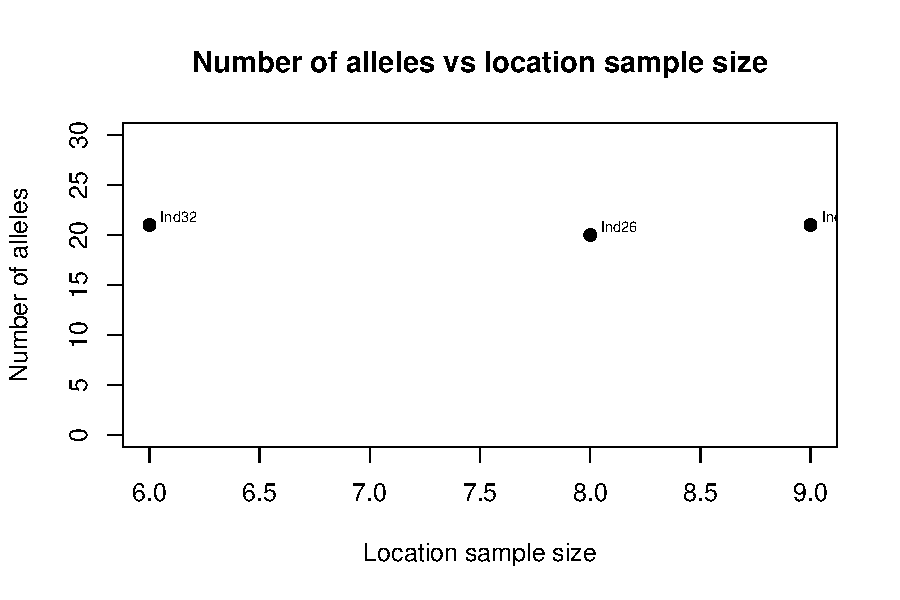
\includegraphics[width=\maxwidth]{PopGenReport-pop_sampsz_vs_alleles-1} 

\end{knitrout}
\FloatBarrier
\noindent
\newline The number of alleles per locus (across all subpopulations):


% latex table generated in R 4.0.4 by xtable 1.8-4 package
% Thu Apr 29 13:49:15 2021
\begin{table}[ht]
\centering
\begin{tabular}{llllll}
   \hline
locus & Locus01 & Locus02 & Locus03 & Locus04 & Locus05 \\ 
   \rowcolor[gray]{0.9} \# alleles & 6 & 8 & 4 & 7 & 5 \\ 
   \hline
\end{tabular}
\caption{Number of alleles per locus across all subpopulations} 
\end{table}







\FloatBarrier
\section{Population-wide test for heterozygosity}

\noindent




% latex table generated in R 4.0.4 by xtable 1.8-4 package
% Thu Apr 29 13:49:15 2021
\begin{table}[ht]
\centering
\begin{tabular}{lrrr}
  \hline
Locus & Expected & Observed & \% difference \\ 
  \hline
Locus01 & 0.707 & 0.719 & -1.728 \\ 
   \rowcolor[gray]{0.9} Locus02 & 0.668 & 0.594 & 11.176 \\ 
  Locus03 & 0.567 & 0.562 & 0.775 \\ 
   \rowcolor[gray]{0.9} Locus04 & 0.725 & 0.781 & -7.817 \\ 
  Locus05 & 0.616 & 0.625 & -1.507 \\ 
   \rowcolor[gray]{0.9}  \hline
\end{tabular}
\caption{The population-wide expected and observed heterozygosity and percent difference ((E-O)/E*100) at each locus} 
\end{table}

\noindent
Bartlett test of homogeneity of variance. This test compares observed vs. expected heterozygosity. A significant result indicates that the population departs from HWE. \\
Bartlett's K-squared: 0.393, df = 1, p-value = 0.5309



\FloatBarrier
\section{Distribution of alleles by subpopulation and loci}
\subsection{Allele frequency plots for all subpopulations and loci}


\FloatBarrier
\begin{knitrout}
\definecolor{shadecolor}{rgb}{0.969, 0.969, 0.969}\color{fgcolor}
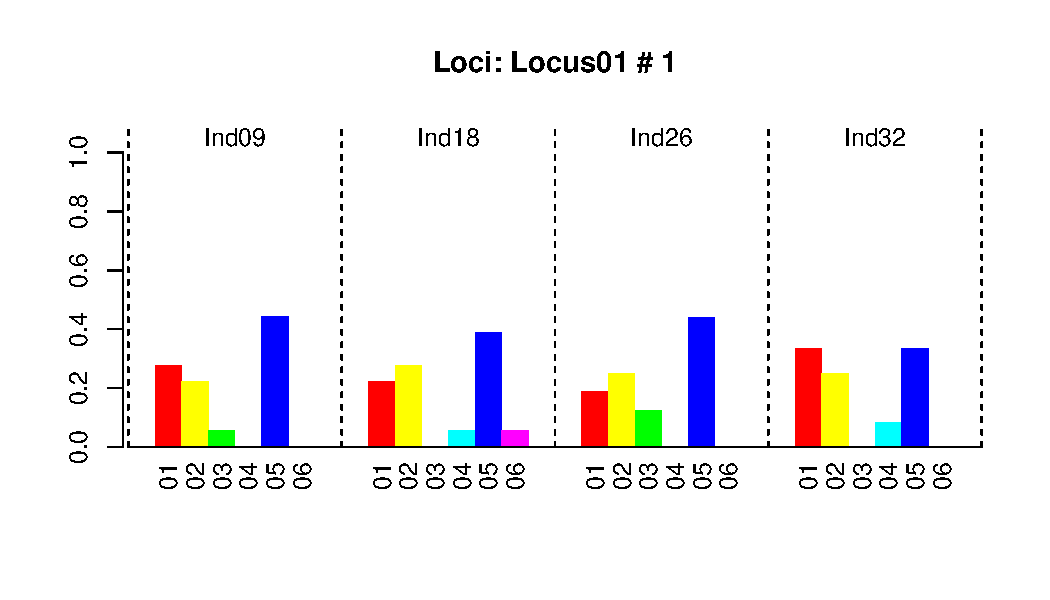
\includegraphics[width=\maxwidth]{PopGenReport-allelfreq-1} 

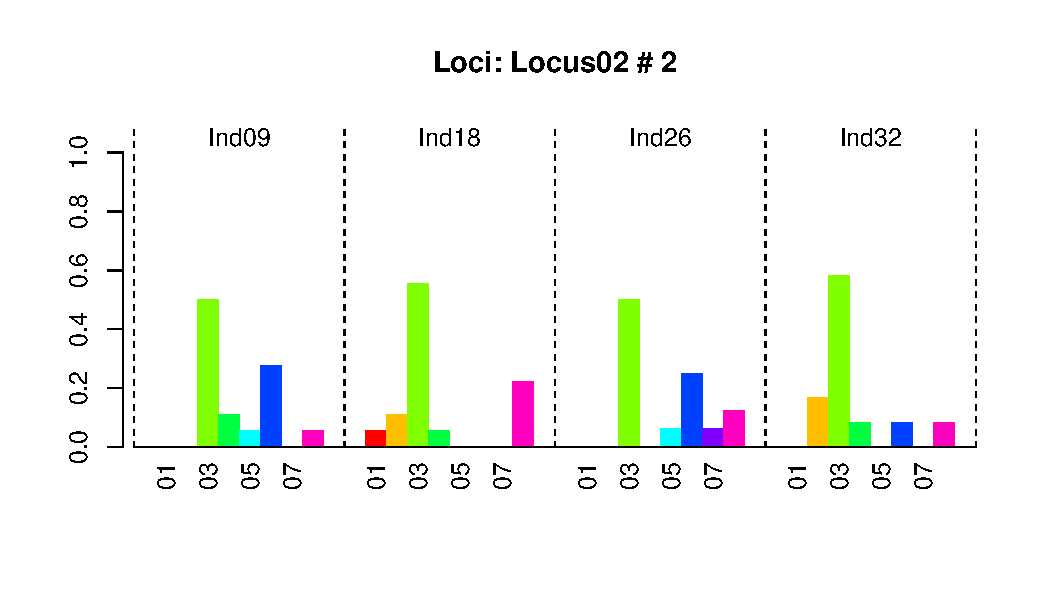
\includegraphics[width=\maxwidth]{PopGenReport-allelfreq-2} 

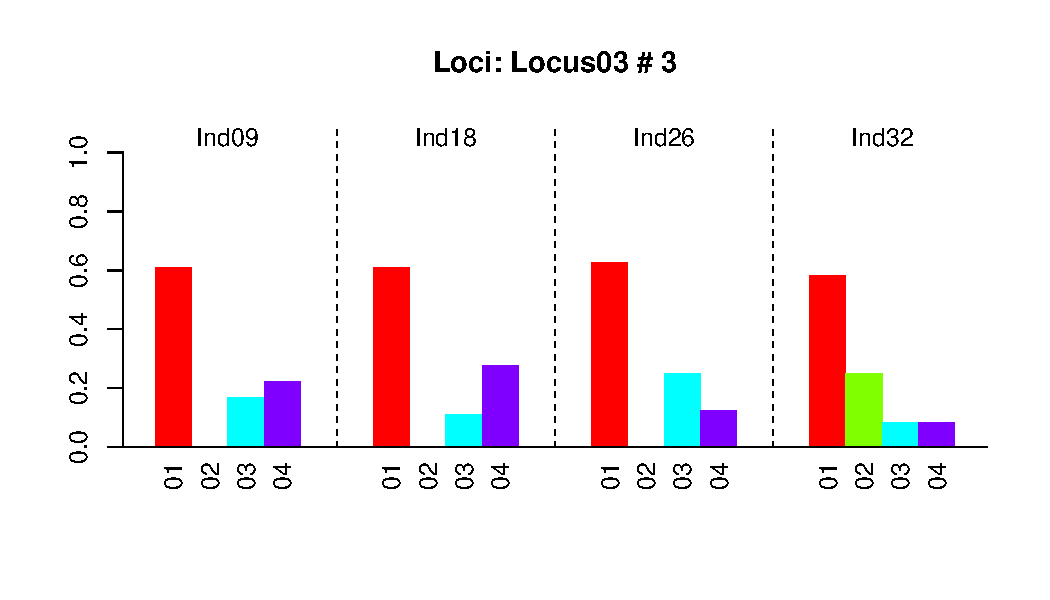
\includegraphics[width=\maxwidth]{PopGenReport-allelfreq-3} 

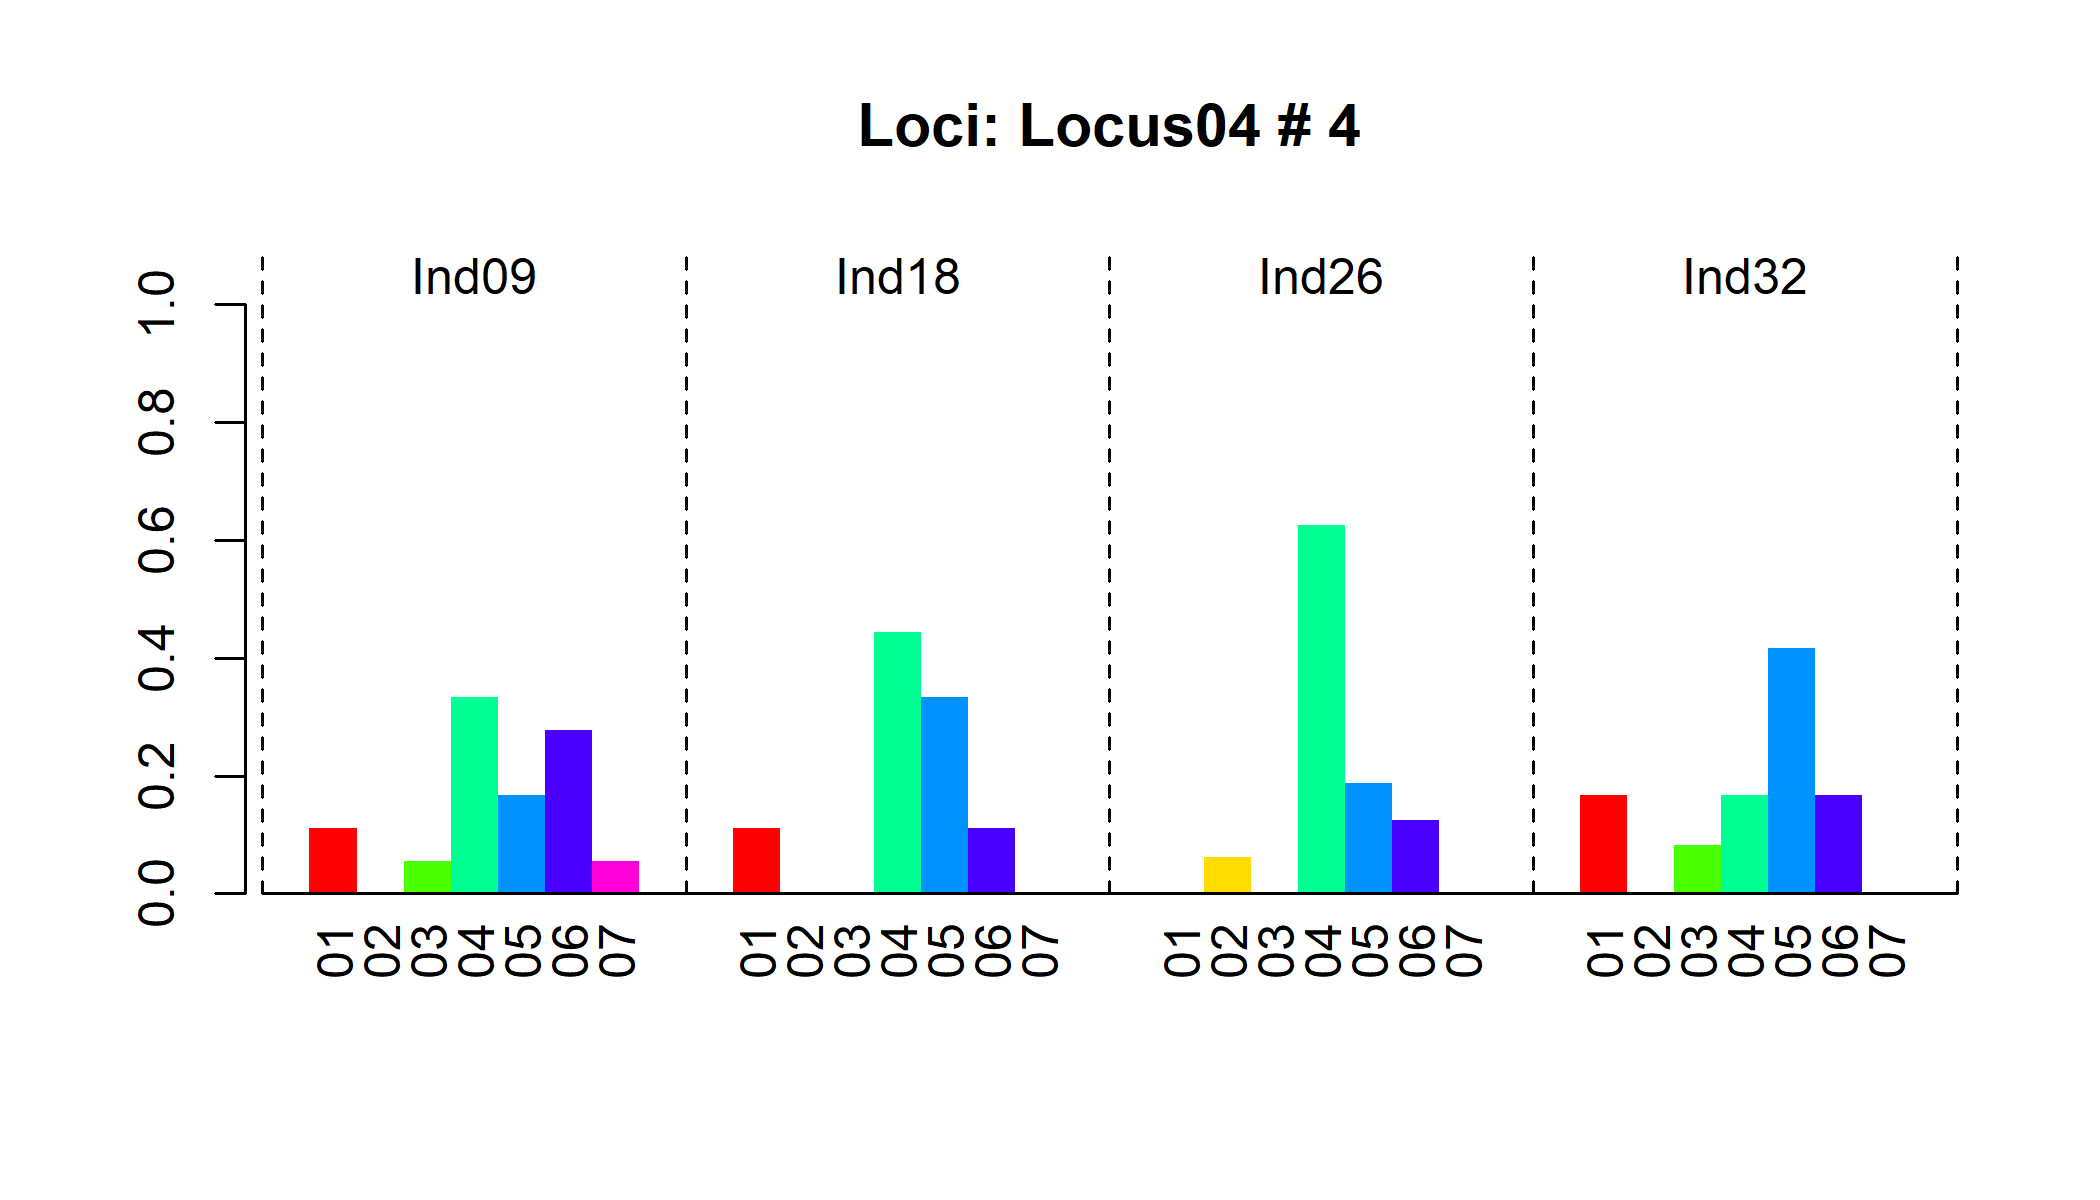
\includegraphics[width=\maxwidth]{PopGenReport-allelfreq-4} 

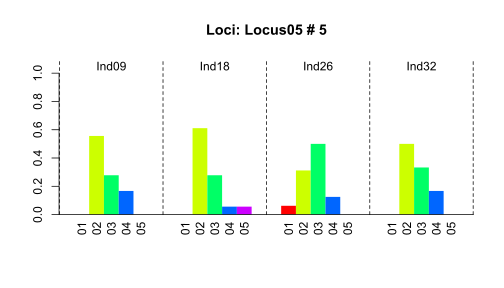
\includegraphics[width=\maxwidth]{PopGenReport-allelfreq-5} 

\end{knitrout}
\FloatBarrier 
\subsection{Heatmaps of allele frequencies for all subpopulation and loci}
Cell colors indicate the proportion of the the total number of alleles in a subpopulation (e.g. 2N) that are of a particular allele type. The numbers within a cell are the counts of the number of alleles in a particular population.  


\FloatBarrier
\begin{knitrout}
\definecolor{shadecolor}{rgb}{0.969, 0.969, 0.969}\color{fgcolor}\begin{figure}
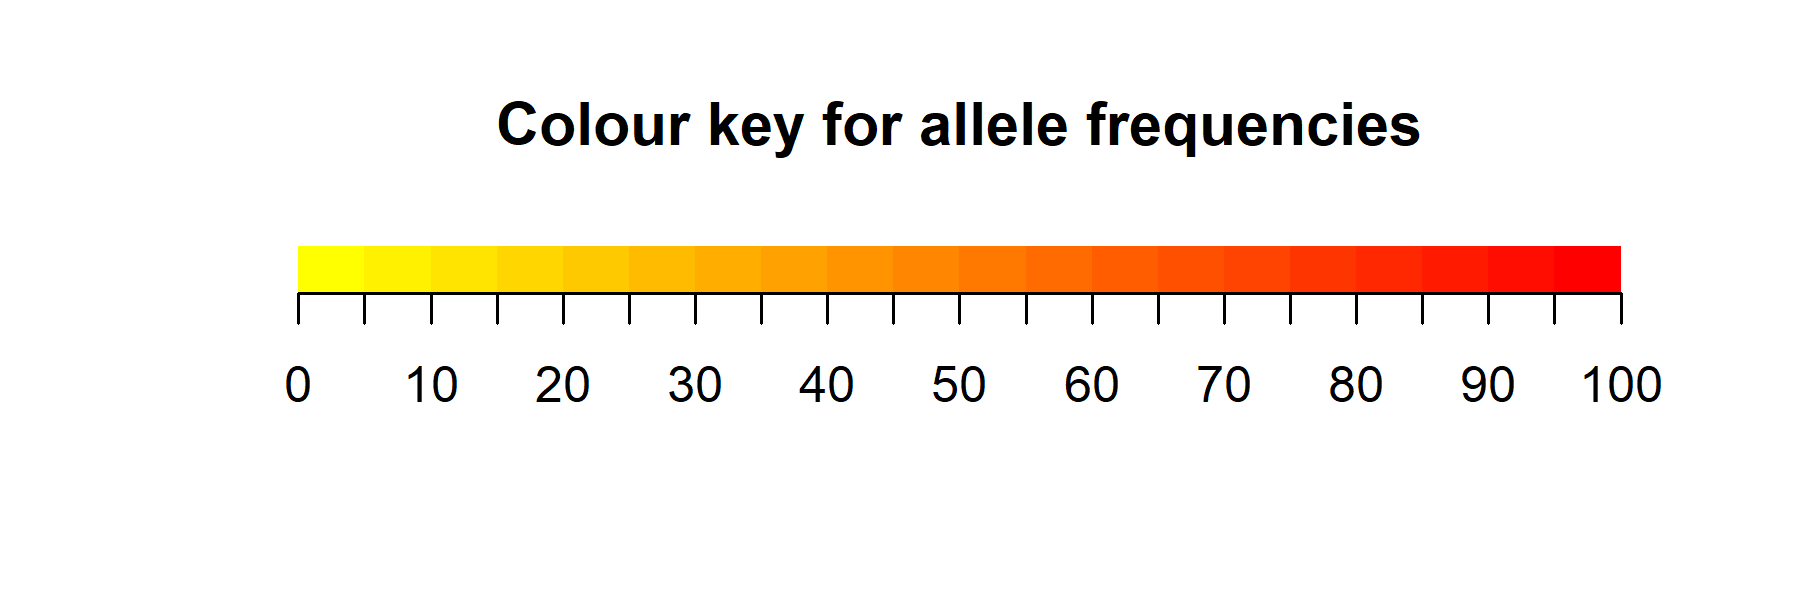
\includegraphics[width=\maxwidth]{PopGenReport-keyall-1} \caption[Color indicates the proportion of the total number of alleles in a subpopulation]{Color indicates the proportion of the total number of alleles in a subpopulation}\label{fig:keyall}
\end{figure}


\end{knitrout}

\FloatBarrier
\begin{knitrout}
\definecolor{shadecolor}{rgb}{0.969, 0.969, 0.969}\color{fgcolor}
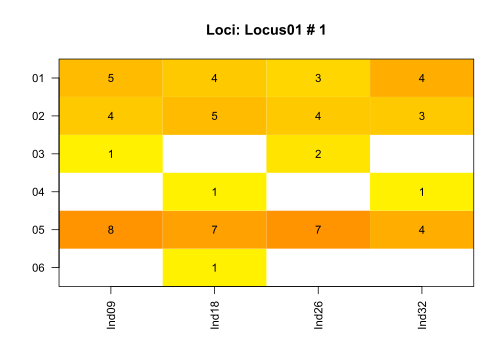
\includegraphics[width=\maxwidth]{PopGenReport-heatmap-1} 

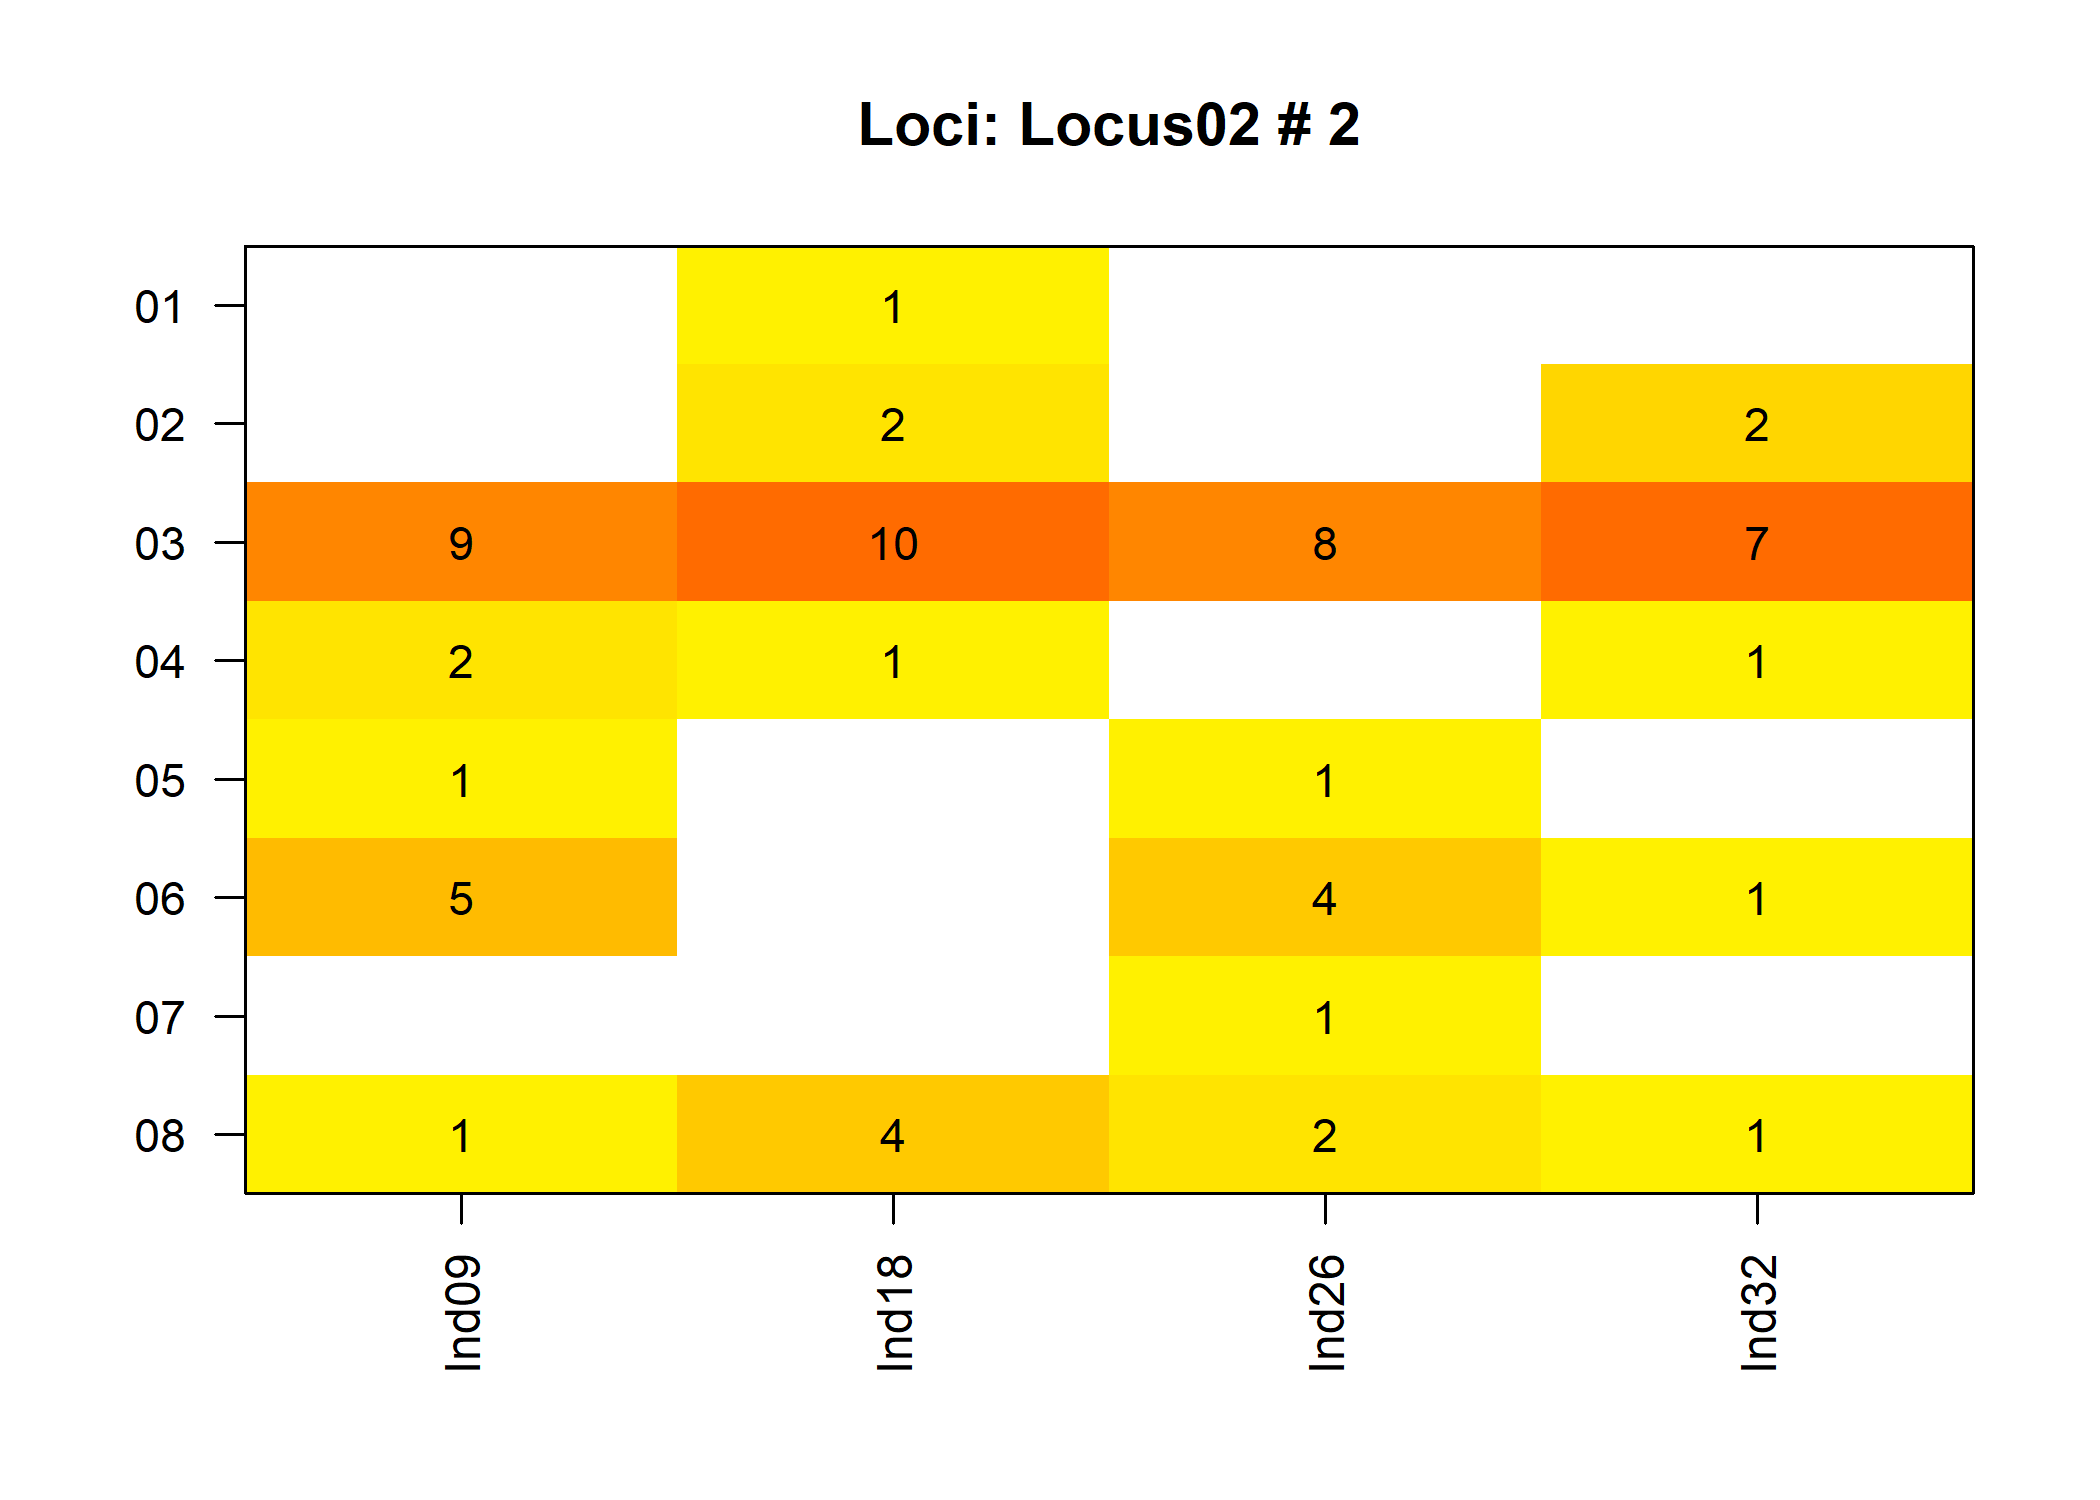
\includegraphics[width=\maxwidth]{PopGenReport-heatmap-2} 

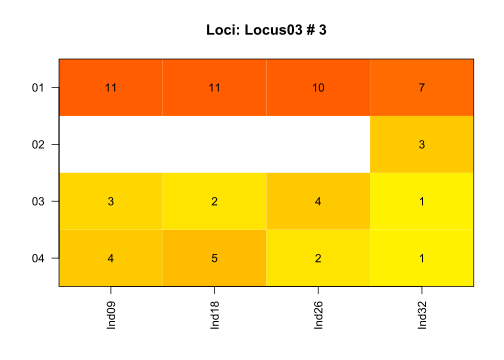
\includegraphics[width=\maxwidth]{PopGenReport-heatmap-3} 

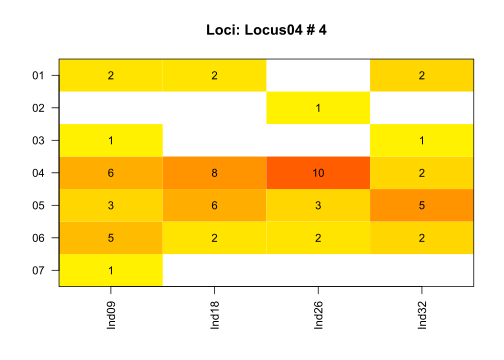
\includegraphics[width=\maxwidth]{PopGenReport-heatmap-4} 

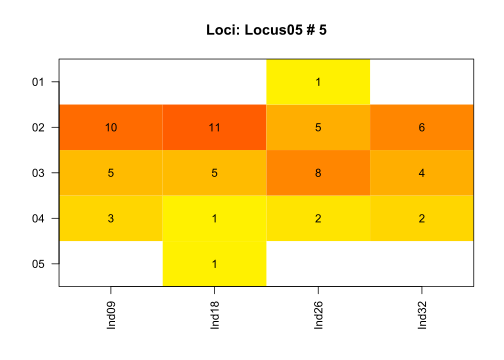
\includegraphics[width=\maxwidth]{PopGenReport-heatmap-5} 

\end{knitrout}
\FloatBarrier

\subsection{Private Alleles}

\FloatBarrier
\subsubsection{All private alleles}
% latex table generated in R 4.0.4 by xtable 1.8-4 package
% Thu Apr 29 13:49:29 2021
\begin{table}[ht]
\centering
\begin{tabular}{lll}
  \hline
Locus & Population & Allele \\ 
  \hline
Locus01 & Ind18 & 06 \\ 
  Locus02 & Ind18 & 01 \\ 
  Locus02 & Ind26 & 07 \\ 
  Locus03 & Ind32 & 02 \\ 
  Locus04 & Ind26 & 02 \\ 
  Locus04 & Ind09 & 07 \\ 
  Locus05 & Ind26 & 01 \\ 
  Locus05 & Ind18 & 05 \\ 
   \hline
\end{tabular}
\caption{List of private alleles by locus and population} 
\end{table}

\FloatBarrier
\subsubsection{Number of private alleles by population}
% latex table generated in R 4.0.4 by xtable 1.8-4 package
% Thu Apr 29 13:49:29 2021
\begin{table}[ht]
\centering
\begin{tabular}{rrrrr}
  \hline
 & Ind09 & Ind18 & Ind26 & Ind32 \\ 
  \hline
Number of private alleles &   1 &   3 &   3 &   1 \\ 
   \hline
\end{tabular}
\caption{Number of private alleles by population} 
\end{table}


\FloatBarrier

\FloatBarrier

\FloatBarrier
\section{Calculation of F statistics for each locus across all sampling locations}


% latex table generated in R 4.0.4 by xtable 1.8-4 package
% Thu Apr 29 13:49:29 2021
\begin{table}[ht]
\centering
\begin{tabular}{rrrr}
  \hline
 & Fit & Fst & Fis \\ 
  \hline
Locus01 & -0.0132 & -0.0510 & 0.0359 \\ 
   \rowcolor[gray]{0.9} Locus03 & 0.0186 & -0.0220 & 0.0398 \\ 
  Locus02 & 0.1241 & -0.0164 & 0.1382 \\ 
   \rowcolor[gray]{0.9} Locus05 & -0.0015 & -0.0098 & 0.0083 \\ 
  Locus04 & -0.0560 & 0.0258 & -0.0840 \\ 
   \rowcolor[gray]{0.9}  \hline
\end{tabular}
\caption{Population wide Fit, Fst, and Fst values for each locus. The table is sorted in ascending order based on Fst.} 
\end{table}


\begin{knitrout}
\definecolor{shadecolor}{rgb}{0.969, 0.969, 0.969}\color{fgcolor}\begin{figure}
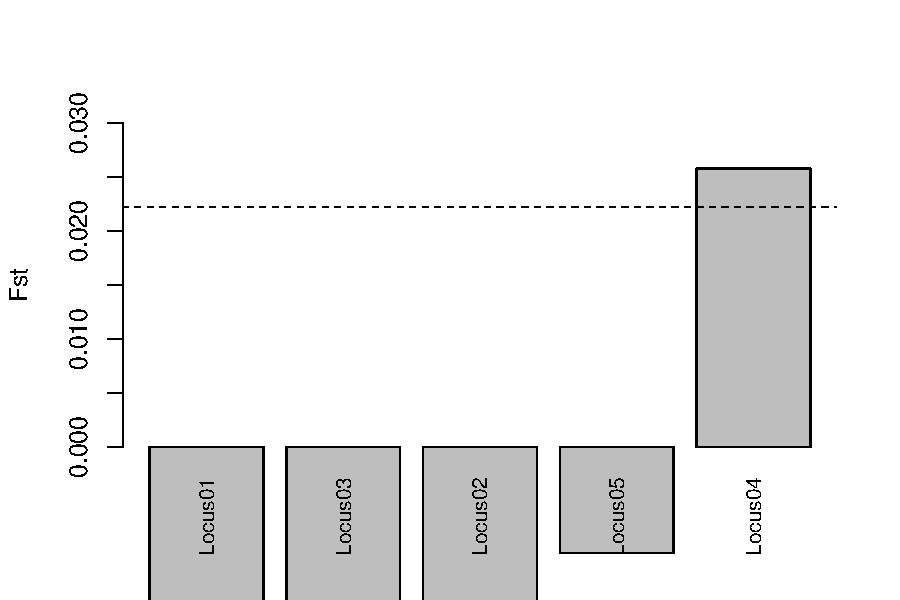
\includegraphics[width=\maxwidth]{PopGenReport-pop_locus_fst-1} \caption[Fst across entire population at each locus]{Fst across entire population at each locus. Solid line shows median Fst, dotted line shows mean Fst, dashed lines indicate 2.5th and 97.5th percentiles of Fst}\label{fig:pop_locus_fst}
\end{figure}


\end{knitrout}
\FloatBarrier

\section{Computation of Nei's pairwise Fst between all pairs of populations}
\begin{knitrout}
\definecolor{shadecolor}{rgb}{0.969, 0.969, 0.969}\color{fgcolor}\begin{kframe}


{\ttfamily\noindent\bfseries\color{errorcolor}{\#\# Error in pairwise.fst(cats, res.type = "{}matrix"{}): could not find function "{}pairwise.fst"{}}}

{\ttfamily\noindent\bfseries\color{errorcolor}{\#\# Error in mat.fst[upper.tri(mat.fst)] <- NA: object 'mat.fst' not found}}

{\ttfamily\noindent\bfseries\color{errorcolor}{\#\# Error in is.data.frame(x): object 'mat.fst' not found}}

{\ttfamily\noindent\bfseries\color{errorcolor}{\#\# Error in xtable(mat.fst, caption = "{}Nei's pairwise Fst between all pairs of populations"{}, : object 'mat.fst' not found}}\end{kframe}
\end{knitrout}



\begin{kframe}


{\ttfamily\noindent\bfseries\color{errorcolor}{\#\# Error in eval(expr, envir, enclos): object 'mat.fst' not found}}\end{kframe}

\begin{knitrout}
\definecolor{shadecolor}{rgb}{0.969, 0.969, 0.969}\color{fgcolor}\begin{kframe}


{\ttfamily\noindent\bfseries\color{errorcolor}{\#\# Error in eval(expr, envir, enclos): object 'mat.fst' not found}}\end{kframe}
\end{knitrout}


\FloatBarrier
\FloatBarrier

\section{Testing for null alleles}




\subsection{Comparison of the observed number of homozygotes vs. expected - overall}
Boxplots show the bootstrap distribution of the expected number of homozygotes for each allele with the boxes showing the 25th (lower edge), 50th (solid line), and 75th (upper edge) percentiles of the distribution and the whiskers showing 1.5 * the inter-quartile range. Solid black dots indicate outliers while red dots indicate the observed number of homozygotes for the allele. If the red dot is above the end of the whisker it suggests that there is an excess of homozygotes for that locus, 

If your results suggest that there is an excess of homozygotes for one (or more) of your loci, you might have a null allele. On the other hand, it could also be incomplete mixing across populations. Try rerunning your analysis by subpopulation or region and see if that resolves the excess of homozygotes. If it doesn't, then you should consider taking more robust measures to check for null alleles. See for instance Girard's (2011) paper on a robust statistical method to detect null alleles.  
\newline
\newline The probability of the observed number of homozygotes for each locus is available in the results object using null.all\$homozygotes\$overall
\begin{knitrout}
\definecolor{shadecolor}{rgb}{0.969, 0.969, 0.969}\color{fgcolor}\begin{kframe}


{\ttfamily\noindent\bfseries\color{errorcolor}{\#\# Error in factor(X2): object 'X2' not found}}\end{kframe}\begin{figure}

\includegraphics[width=\maxwidth]{PopGenReport-null_all_overall_ho-1} \caption[Number of observed homozygotes at each locus (red dots) compared to the distribution of the expected number of homozygotes assuming HWE (boxplots)]{Number of observed homozygotes at each locus (red dots) compared to the distribution of the expected number of homozygotes assuming HWE (boxplots)}\label{fig:null_all_overall_ho}
\end{figure}


\end{knitrout}
\FloatBarrier

\subsection{Comparison of the observed number of homozygotes vs. expected - by locus}
Boxplots show the bootstrap distribution of the expected number of homozygotes for each allele with the boxes showing the 25th (lower edge), 50th (solid line), and 75th (upper edge) percentiles of the distribution and the whiskers showing 1.5 * the inter-quartile range. Solid black dots indicate outliers while red dots indicate the observed number of homozygotes for the allele. If the red dot is above the end of the whisker it suggests that there is an excess of homozygotes for that allele. 
\newline
\newline The probability of the observed number of homozygotes for each allele is available in the results object using null.all\$homozygotes\$probability.obs

\noindent
\begin{knitrout}
\definecolor{shadecolor}{rgb}{0.969, 0.969, 0.969}\color{fgcolor}
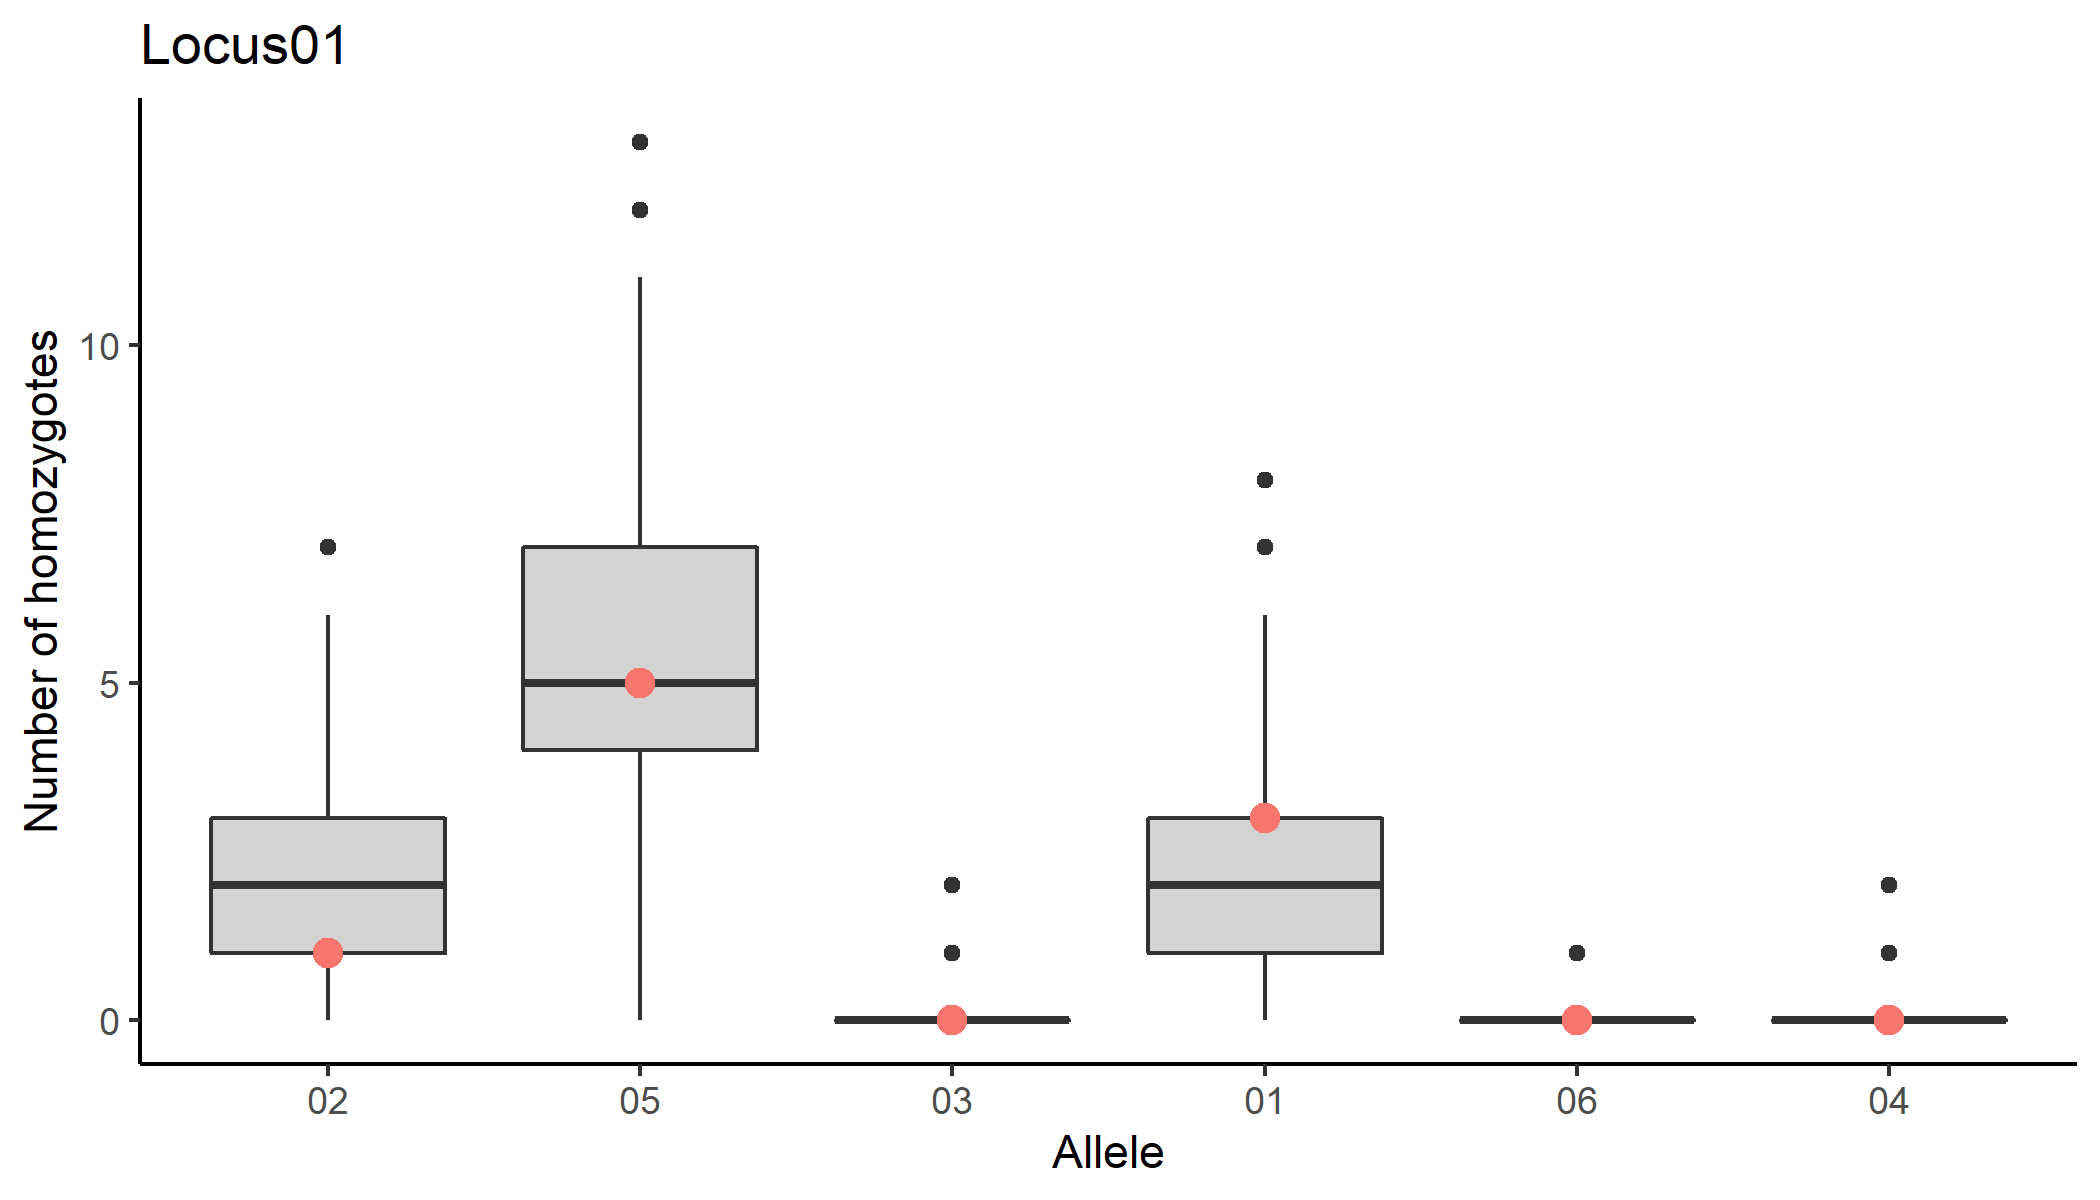
\includegraphics[width=\maxwidth]{PopGenReport-null_all-1} 

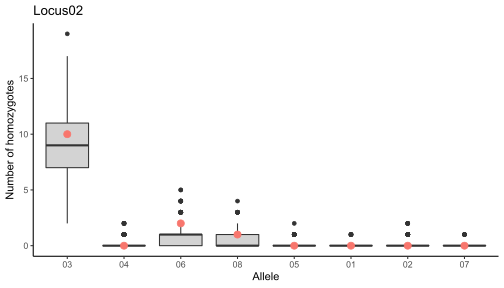
\includegraphics[width=\maxwidth]{PopGenReport-null_all-2} 

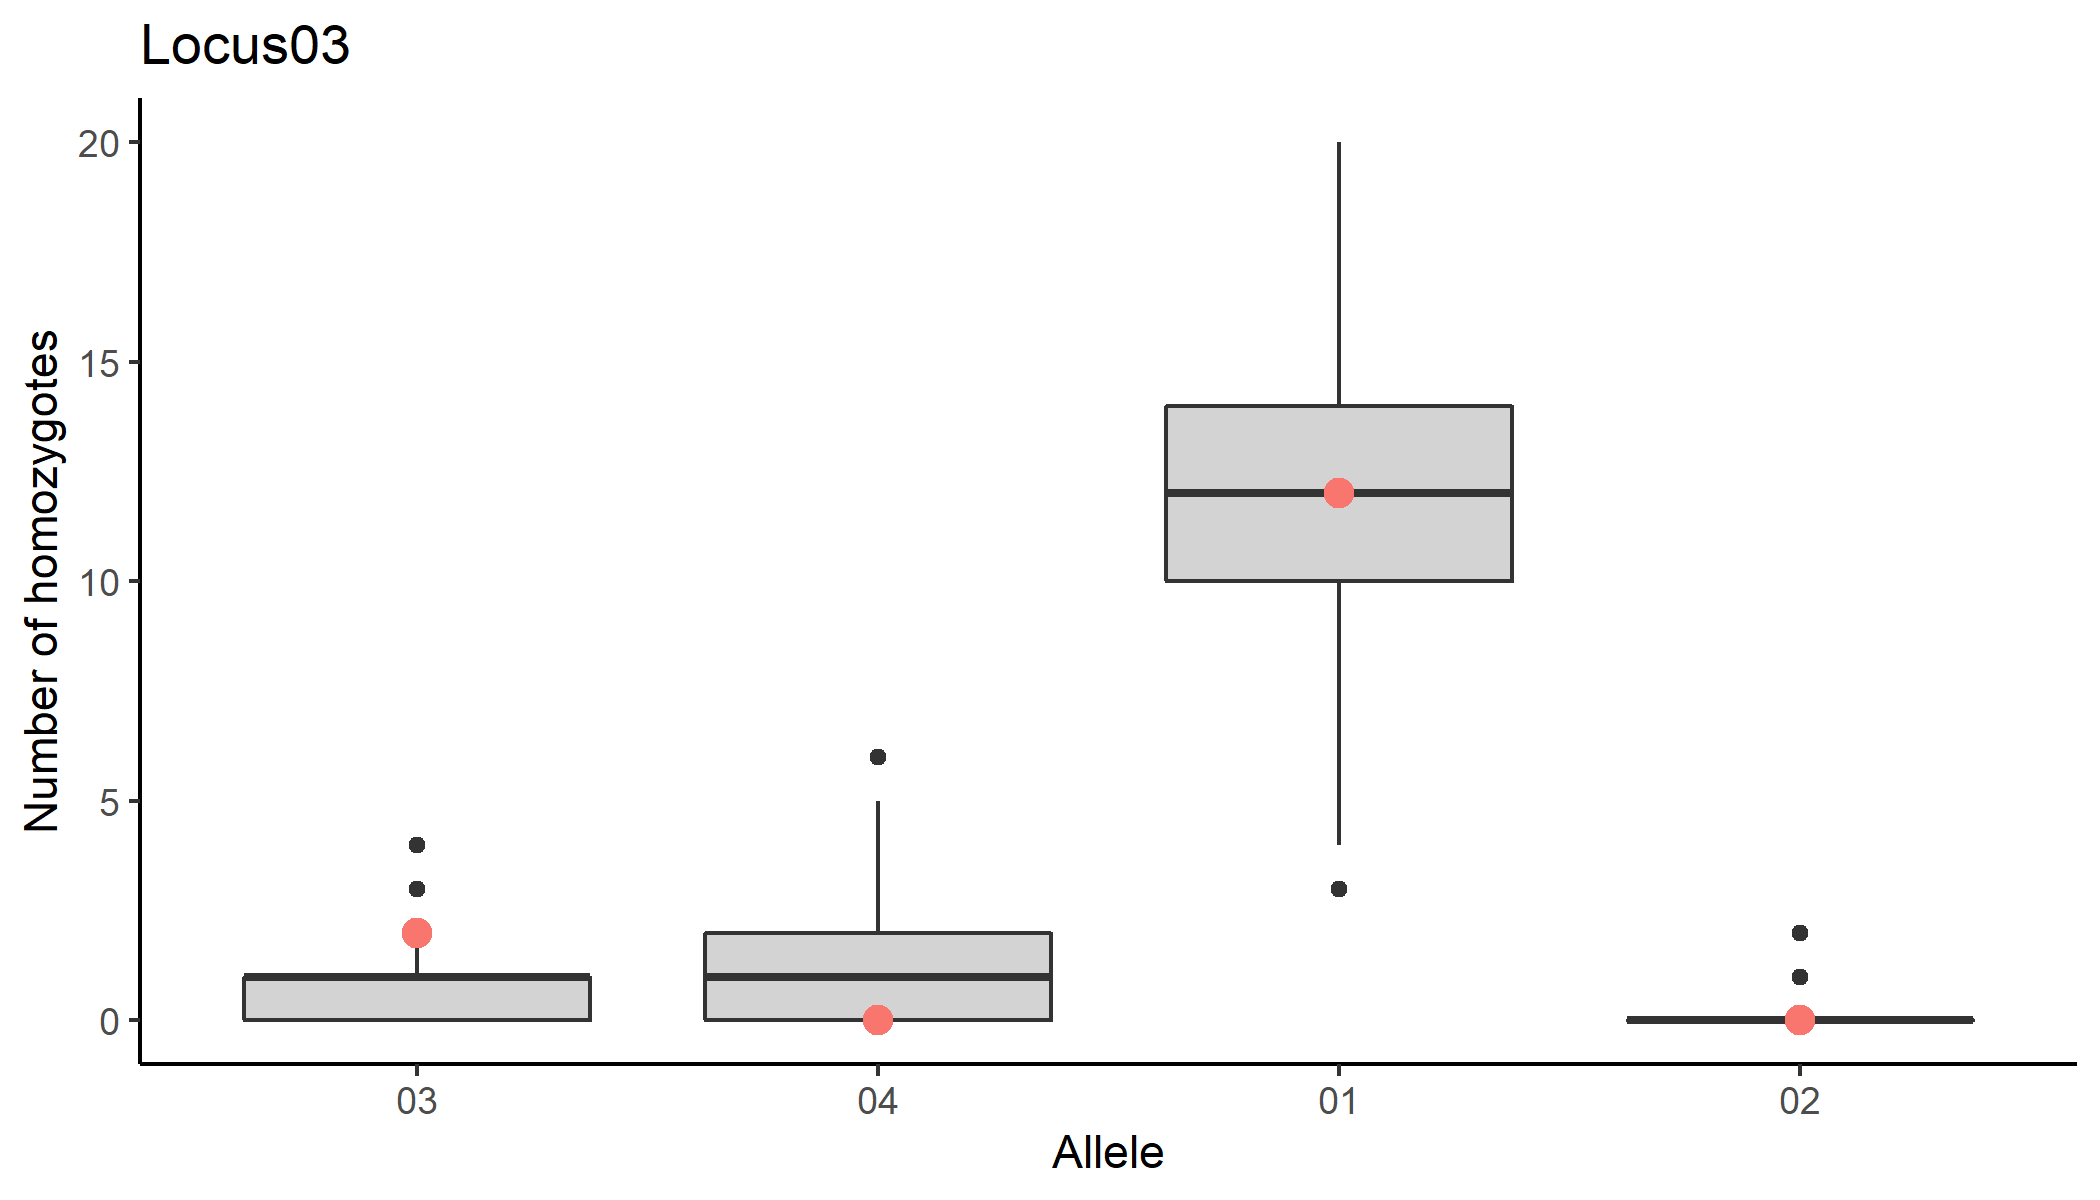
\includegraphics[width=\maxwidth]{PopGenReport-null_all-3} 

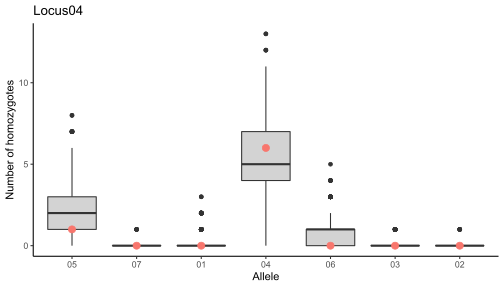
\includegraphics[width=\maxwidth]{PopGenReport-null_all-4} 

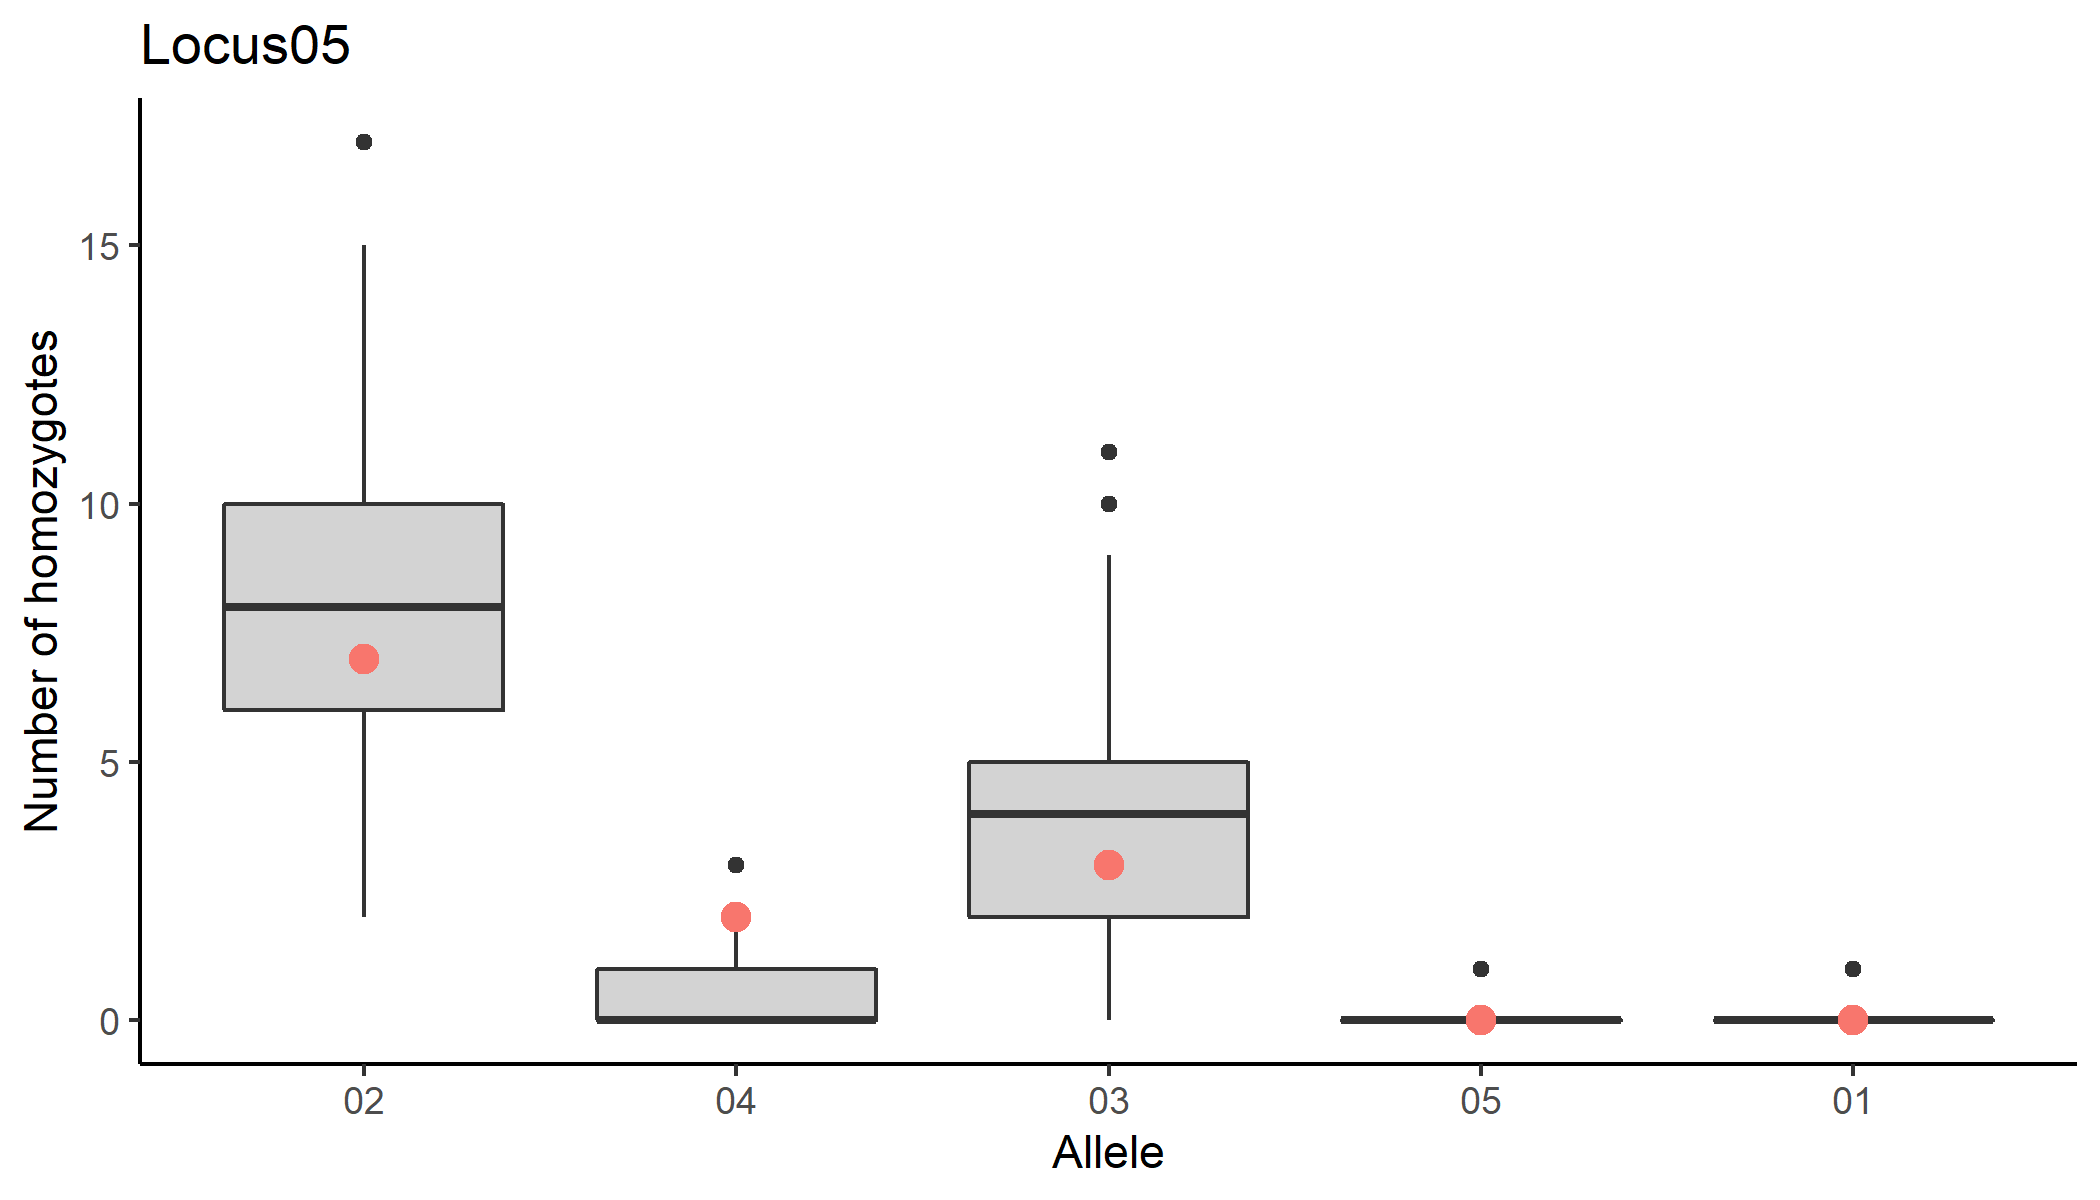
\includegraphics[width=\maxwidth]{PopGenReport-null_all-5} 

\end{knitrout}

% latex table generated in R 4.0.4 by xtable 1.8-4 package
% Thu Apr 29 13:49:49 2021
\begin{table}[ht]
\centering
\begin{tabular}{rrrrrrrrr}
  \hline
 & Allele-1 & Allele-2 & Allele-3 & Allele-4 & Allele-5 & Allele-6 & Allele-7 & Allele-8 \\ 
  \hline
Locus01 & 0.607 & 0.417 & 0.071 & 0.145 & 0.015 & 0.031 &  &  \\ 
   \rowcolor[gray]{0.9} Locus02 & 0.255 & 0.102 & 0.036 & 0.076 & 0.036 & 0.007 & 0.119 & 0.006 \\ 
  Locus03 & 0.044 & 0.661 & 0.413 & 0.075 &  &  &  &  \\ 
   \rowcolor[gray]{0.9} Locus04 & 0.676 & 0.006 & 0.240 & 0.286 & 0.597 & 0.034 & 0.006 &  \\ 
  Locus05 & 0.568 & 0.020 & 0.523 & 0.004 & 0.012 &  &  &  \\ 
   \rowcolor[gray]{0.9}  \hline
\end{tabular}
\caption{Probability of the observed number of homozygotes} 
\end{table}


\FloatBarrier

\subsection{Frequency of null alleles}
\subsubsection{Determined using Chakraborty et al. (1992)}


\begin{knitrout}
\definecolor{shadecolor}{rgb}{0.969, 0.969, 0.969}\color{fgcolor}
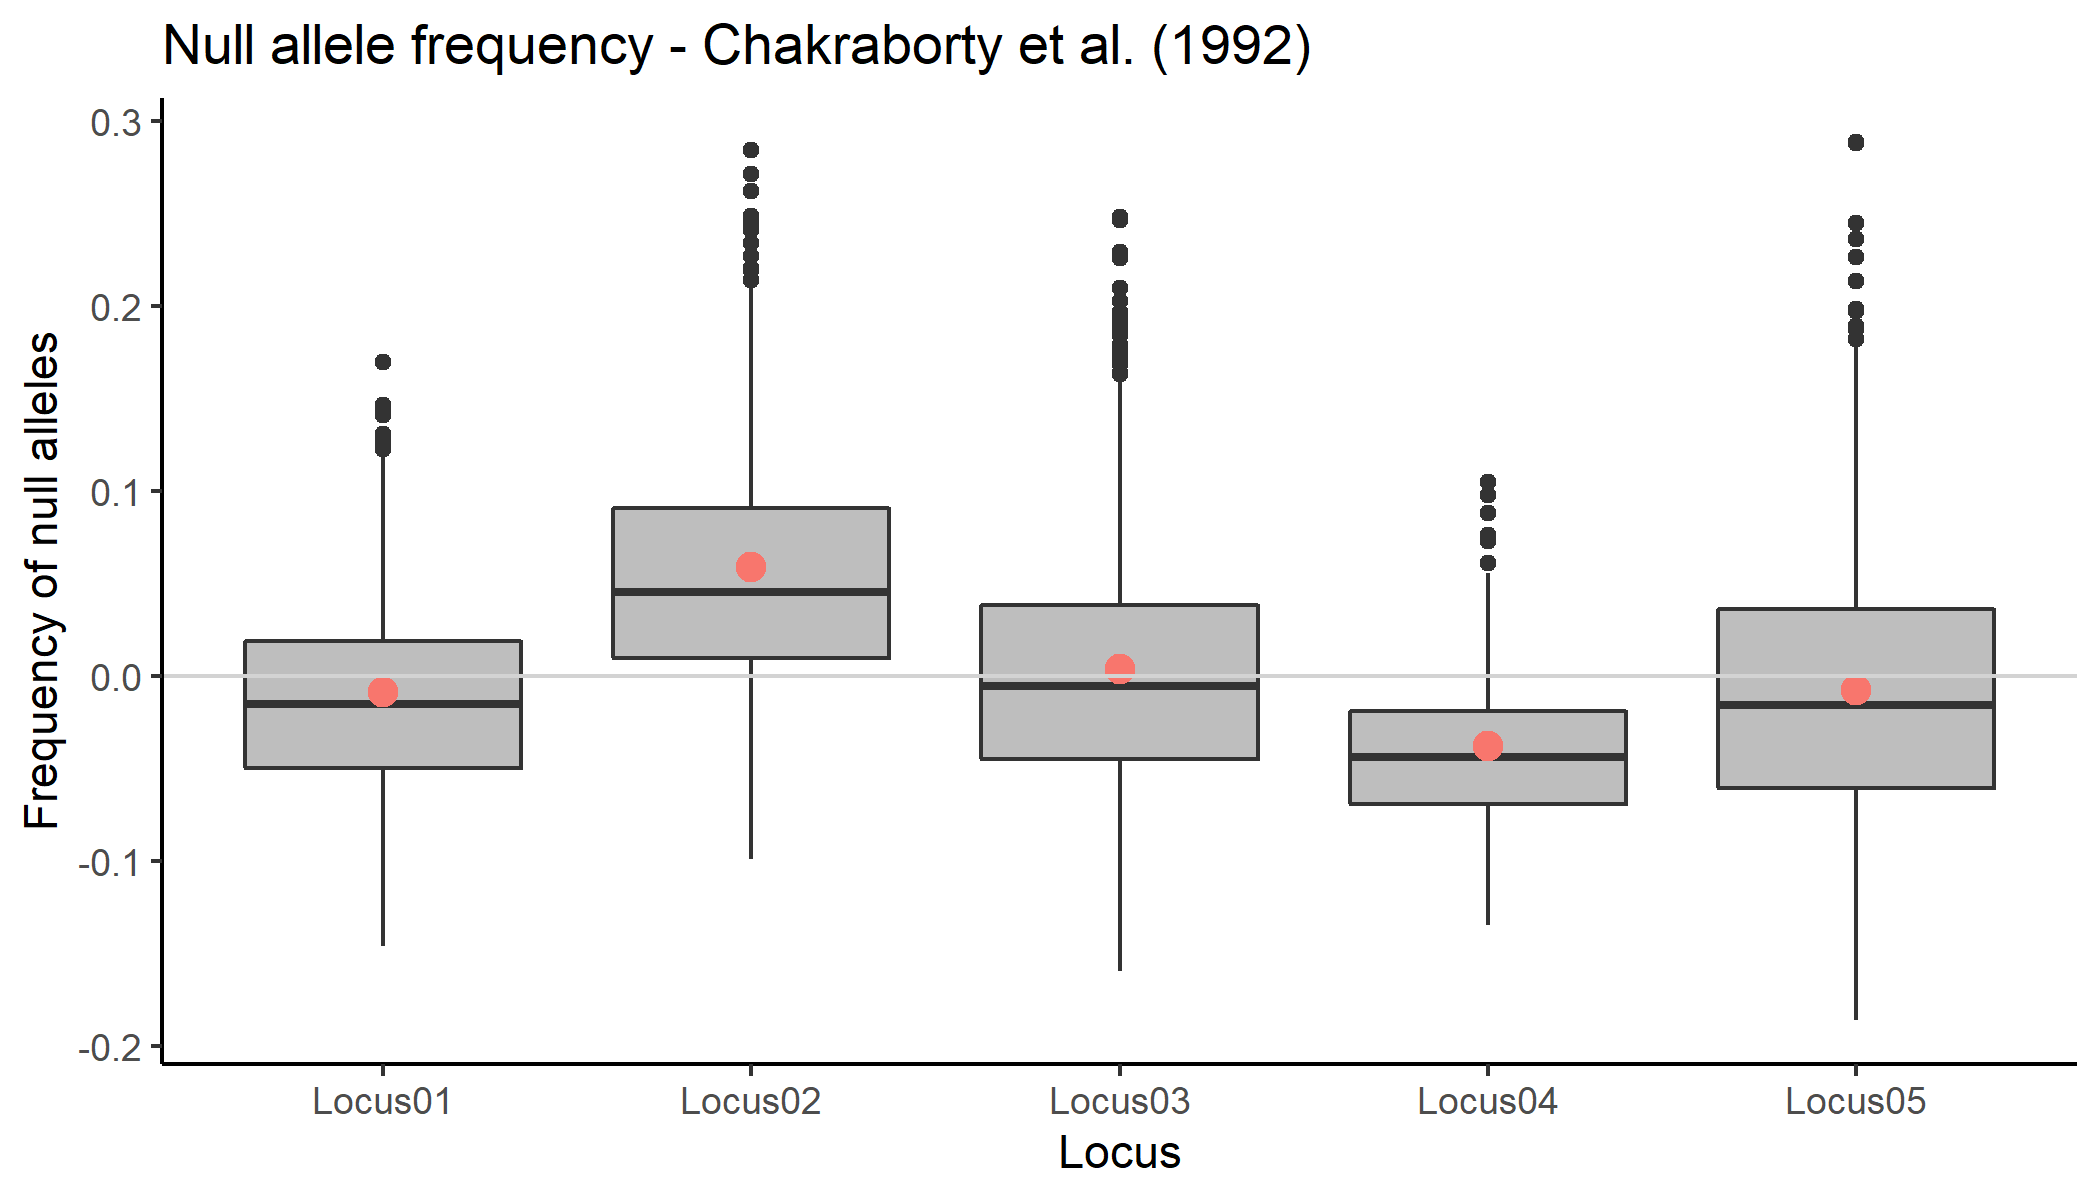
\includegraphics[width=\maxwidth]{PopGenReport-null_all_Chakraborty-1} 

\end{knitrout}




\subsubsection{Determined using Brookfield (1996)}


\begin{knitrout}
\definecolor{shadecolor}{rgb}{0.969, 0.969, 0.969}\color{fgcolor}
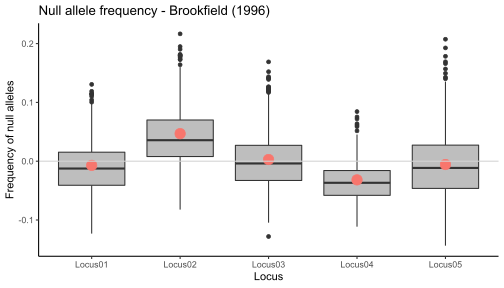
\includegraphics[width=\maxwidth]{PopGenReport-null_all_Brookfield-1} 

\end{knitrout}


% latex table generated in R 4.0.4 by xtable 1.8-4 package
% Thu Apr 29 13:49:53 2021
\begin{table}[ht]
\centering
\begin{tabular}{rrrrrr}
  \hline
 & Locus01 & Locus02 & Locus03 & Locus04 & Locus05 \\ 
  \hline
Observed frequency & -0.007 & 0.047 & 0.003 & -0.032 & -0.006 \\ 
  Median frequency & -0.012 & 0.036 & -0.004 & -0.037 & -0.011 \\ 
  2.5th percentile & -0.094 & -0.042 & -0.075 & -0.090 & -0.112 \\ 
  97.5th percentile & 0.076 & 0.140 & 0.100 & 0.027 & 0.110 \\ 
   \hline
\end{tabular}
\caption{Summary of null allele frequencies by locus for Brookfield (1996)} 
\end{table}


\FloatBarrier

\FloatBarrier


\section{Allelic richness}



Allelic richness for each locus and subpopulation was based on a subsample of {12} alleles.

% latex table generated in R 4.0.4 by xtable 1.8-4 package
% Thu Apr 29 13:49:54 2021
\begin{table}[ht]
\centering
\begin{tabular}{rrrrr}
  \hline
 & Ind09 & Ind18 & Ind26 & Ind32 \\ 
  \hline
Locus01 & 3.530 & 4.091 & 3.810 & 3.753 \\ 
   \rowcolor[gray]{0.9} Locus02 & 3.936 & 3.919 & 4.087 & 4.236 \\ 
  Locus03 & 2.907 & 2.812 & 2.853 & 3.515 \\ 
   \rowcolor[gray]{0.9} Locus04 & 4.864 & 3.637 & 3.439 & 4.621 \\ 
  Locus05 & 2.923 & 3.116 & 3.479 & 2.953 \\ 
   \rowcolor[gray]{0.9}  \hline
\end{tabular}
\caption{Allelic richness by locus and population} 
\end{table}
% latex table generated in R 4.0.4 by xtable 1.8-4 package
% Thu Apr 29 13:49:54 2021
\begin{table}[ht]
\centering
\begin{tabular}{rrrrr}
  \hline
 & Ind09 & Ind18 & Ind26 & Ind32 \\ 
  \hline
Mean richness & 3.632 & 3.515 & 3.534 & 3.815 \\ 
   \rowcolor[gray]{0.9} Total richness & 18.160 & 17.575 & 17.670 & 19.077 \\ 
   \hline
\end{tabular}
\caption{Allelic richness summary statistics} 
\end{table}




\FloatBarrier


\section{Hs and Ht based population differentiation statistics}



% latex table generated in R 4.0.4 by xtable 1.8-4 package
% Thu Apr 29 13:49:55 2021
\begin{table}[ht]
\centering
\begin{tabular}{rrrrrr}
  \hline
 & Hs & Ht & Gst & Gprime\_st & D \\ 
  \hline
Locus01 & 0.746 & 0.720 & -0.036 & -0.192 & -0.136 \\ 
   \rowcolor[gray]{0.9} Locus02 & 0.682 & 0.677 & -0.008 & -0.032 & -0.022 \\ 
  Locus03 & 0.588 & 0.582 & -0.011 & -0.036 & -0.021 \\ 
   \rowcolor[gray]{0.9} Locus04 & 0.727 & 0.741 & 0.019 & 0.092 & 0.069 \\ 
  Locus05 & 0.634 & 0.628 & -0.010 & -0.036 & -0.023 \\ 
   \rowcolor[gray]{0.9}  \hline
\end{tabular}
\caption{Hs and Ht based estimates of differentiation: Gst, Gst and Dest for each locus} 
\end{table}
% latex table generated in R 4.0.4 by xtable 1.8-4 package
% Thu Apr 29 13:49:55 2021
\begin{table}[ht]
\centering
\begin{tabular}{rrrrrr}
  \hline
Hs & Ht & Gst\_est & Gprime\_st & D\_het & D\_mean \\ 
  \hline
0.676 & 0.670 & -0.009 & -0.037 & -0.024 &  \\ 
   \rowcolor[gray]{0.9}  \hline
\end{tabular}
\caption{Hs and Ht based global estimates of differentiation: Gst, Gst and Dest for each locus} 
\end{table}





% latex table generated in R 4.0.4 by xtable 1.8-4 package
% Thu Apr 29 13:49:56 2021
\begin{table}[ht]
\centering
\begin{tabular}{rrrrr}
  \hline
 & Ind09 & Ind18 & Ind26 & Ind32 \\ 
  \hline
Ind09 &  &  &  &  \\ 
  Ind18 & -0.038 &  &  &  \\ 
  Ind26 & -0.030 & 0.001 &  &  \\ 
  Ind32 & -0.058 & -0.059 & 0.032 &  \\ 
   \hline
\end{tabular}
\caption{mmod Jost's D pairwise} 
\end{table}
% latex table generated in R 4.0.4 by xtable 1.8-4 package
% Thu Apr 29 13:49:56 2021
\begin{table}[ht]
\centering
\begin{tabular}{rrrrr}
  \hline
 & Ind09 & Ind18 & Ind26 & Ind32 \\ 
  \hline
Ind09 &  &  &  &  \\ 
  Ind18 & -0.057 &  &  &  \\ 
  Ind26 & -0.045 & 0.002 &  &  \\ 
  Ind32 & -0.085 & -0.089 & 0.046 &  \\ 
   \hline
\end{tabular}
\caption{Pairwise Gst - Hedrick} 
\end{table}
% latex table generated in R 4.0.4 by xtable 1.8-4 package
% Thu Apr 29 13:49:56 2021
\begin{table}[ht]
\centering
\begin{tabular}{rrrrr}
  \hline
 & Ind09 & Ind18 & Ind26 & Ind32 \\ 
  \hline
Ind09 &  &  &  &  \\ 
  Ind18 & -0.009 &  &  &  \\ 
  Ind26 & -0.007 & 0.000 &  &  \\ 
  Ind32 & -0.013 & -0.014 & 0.007 &  \\ 
   \hline
\end{tabular}
\caption{Pairwise Gst - Nei} 
\end{table}





\FloatBarrier
\section{Testing for HWE for each combination of location and locus}


\subsection{Testing HWE for each combination of location and locus}



\noindent
The table below shows the p-value for the test of HWE for each combination of location and locus. The p-values shown here differ from those produced by GENALEX as the Chi-square test performed here includes the Yates continuity correction which GENALEX does not. As a large number of Chi-square tests are performed, $\alpha$ = 0.05  cannot be used as Type I errors are likely to occur. Instead a Bonferroni adjustment is used $\alpha$ = (0.05/ 20) = 0.0025.

% latex table generated in R 4.0.4 by xtable 1.8-4 package
% Thu Apr 29 13:49:58 2021
\begin{table}[ht]
\centering
\begin{tabular}{rrrrr}
  \hline
 & Ind09 & Ind18 & Ind26 & Ind32 \\ 
  \hline
Locus01 & 0.940 & 0.311 & 0.076 & 1.000 \\ 
   \rowcolor[gray]{0.9} Locus02 & 0.351 & 0.810 & 0.207 & 1.000 \\ 
  Locus03 & 0.069 & 0.195 & 0.702 & 1.000 \\ 
   \rowcolor[gray]{0.9} Locus04 & 0.468 & 1.000 & 0.304 & 0.372 \\ 
  Locus05 & 0.251 & 0.094 & 0.224 & 0.095 \\ 
   \rowcolor[gray]{0.9}  \hline
\end{tabular}
\caption{Chi-square test of HWE p-values for each combination of location and locus} 
\end{table}






\FloatBarrier

\subsection{Combinations of location and locus that depart from HWE}

There were no departures from HWE for any combination of sub-population and locus



\FloatBarrier
\section{Principal Coordinate Analysis}

Principal coordinate analysis. This plot, using the first two axes, visualises genetic diversity among sampled individuals. Missing data are replaced by the mean of the allele frequencies.
Colors indicate subpopulation if specified in the genetic data set.


\begin{knitrout}
\definecolor{shadecolor}{rgb}{0.969, 0.969, 0.969}\color{fgcolor}
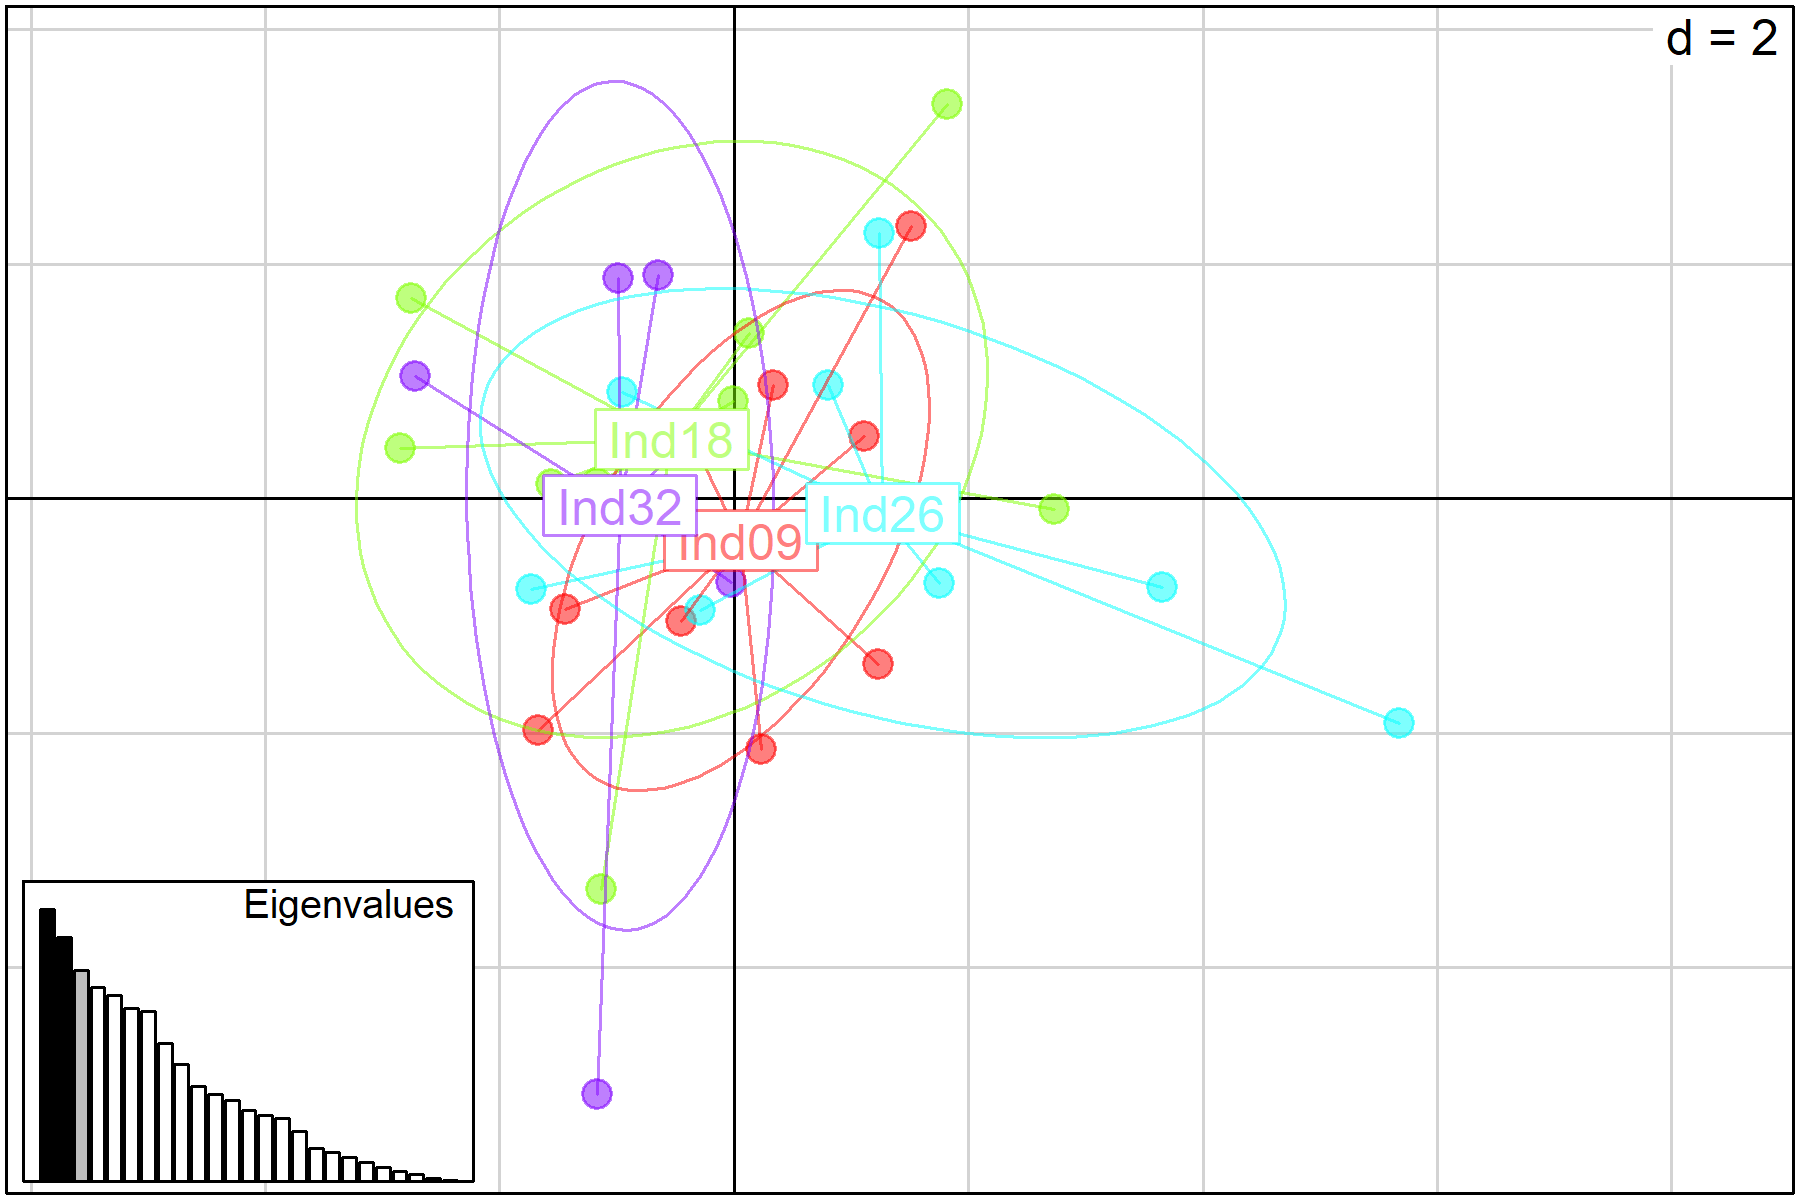
\includegraphics[width=\maxwidth]{PopGenReport-pcoa-1} 

\end{knitrout}

\FloatBarrier
\end{document}
